\scanpage{9}
1) \uline{Ens. avec permutation} $(E,u)\Longleftrightarrow\mathbb{Z}$-ens.

Classification : famille de cardinaux associés aux ss-groupes de $\mathbb{Z}$
\[
=\text{famille de cardinaux}\quad
\begin{tikzpicture}[baseline=-1ex]
\draw[gray!55,line width=.2pt] (0,.08)--(.08,-.10);
\draw[gray!80,line width=.35pt] (.08,-.10)--(.25,.08);
\node[inner sep=0pt] at (.34,.08) {$\unsure{\phantom{x}}$};
\end{tikzpicture}\quad(a_i)_{i\in\mathbb{N}}
\]

\[
E\ \text{fini}\Longleftrightarrow
\underbrace{n_{0}=0}_{\substack{\text{orbites}\\\text{finies}}}
\ \text{et}\quad
\underbrace{\text{les } n_{i}\ \text{finis}}_{\substack{\text{nb fini d'}\\\text{orbites de}\\\text{cardinal } i\in\mathbb{N}\\\text{donné}}},
\quad\underbrace{\text{nuls sauf un nb fini}}_{\text{nb fini d'orbites}}
\]

$u$ transitif ($\Longleftrightarrow u$ définit sur $E$ un ordre circulaire) $\Leftrightarrow$ tous les $n_{i}$ sauf un au plus sont nuls

\uline{Cor} Les classes d'éléments de $\unsure{\mathfrak{S}|\mathscr{S}}_{n}$ mod conjugaison correspondent $1$-$1$\par
\noindent\begin{tabular}{@{}|@{\hspace{.6em}}p{\dimexpr\linewidth-1em\relax}@{}}
aux ``partitions'' de $n$, i.e. aux familles d'entiers $(c_{i})_{1\leq i\leq n}$ tels que
\[
\makebox[\linewidth][l]{$\displaystyle\sum i c_{i}=n$}
\]
\end{tabular}

\diagram{\resizebox{\linewidth}{!}{\begingroup\setlength{\arraycolsep}{2.5pt}\(\begin{array}{ll l|ll l}
\mathfrak{S}_{2}:&2\ \text{\unsure{classes|classe}}&1,\sigma_{12}&\unsure{\mathfrak{A}|\mathscr{A}}_{2}:&1\ \text{classe}&1\\
\mathfrak{S}_{3}:&3\ \text{classes}&1,\sigma_{12},\sigma_{123}&\mathfrak{A}_{3}:&3\ {-}&1,\sigma_{123},\sigma_{321}\\
\mathfrak{S}_{4}:&5\ \text{classes}&1,\sigma_{12},\sigma_{12}\sigma_{34},\sigma_{123},\sigma_{1234}
&\mathfrak{A}_{4}:&\multicolumn{2}{l}{\tikz[baseline=(entry.base)]{
  \node[inner sep=1.5pt] (entry) {$\deleted{\unsure{1|i},\sigma_{\unsure{12|13}}\sigma_{\unsure{34|24}},\sigma_{\unsure{1234|4234}}}$};
  \draw[rounded corners=2.5pt] ([xshift=-2em,yshift=1.5pt]entry.north east)
    -- ([xshift=-2em]entry.north east) -- (entry.north west) -- (entry.south west)
    -- ([xshift=-1.65em]entry.south east) -- ([xshift=-1.65em,yshift=-1.5pt]entry.south east);
}}\\
\mathfrak{S}_{5}:&?&&&&
\end{array}\)\endgroup}}

2) \uline{Rectification} Les contours orientés correspondent aux ens. à permutation $(E,u)$ tels que $u$ n'\uline{ait pas de pt fixe} (car on ne veut pas de polygone à $1$ coté, ds les graphes !)

3) Produit $\frac{1}{2}$ direct de gpes

\diagram{\begin{tikzcd}[ampersand replacement=\&,column sep=small]
\text{donner}\&[-1ex]1 \arrow[r,dash] \& \mathbb{Z}\arrow[r,dash,"i"] \& G\arrow[r,dash,"p"] \& \Gamma\arrow[l,bend left=24,"q"']\arrow[r,dash] \& 1q \&[-1ex] \unsure{p|q}qp=\operatorname{id}_{\Gamma}\quad\unsure{q|p}
\end{tikzcd}}
(suite exacte, avec $q$ un hom. de \unsure{gpes|groupes})

revient à donner
\diagram{\begin{tikzcd}[ampersand replacement=\&,column sep=small,row sep=0pt]
1\arrow[r,dash] \& Z\arrow[r,dash] \& G\arrow[r] \& \Gamma\arrow[r,dash] \& 1 \& p\mid\Gamma'\simeq\deleted{\unsure{\mathrm{iso}|\mathrm{is}}}\Gamma\ \text{\unsure{iso|is}}\\
\& \& \rotatebox{90}{$\subset$} \\
\& \& \Gamma'
\end{tikzcd}}

ou à donner \unsure{grs|gpes} $Z,\Gamma$ avec op. de $\Gamma$ sur $Z$
\[
\Gamma\longrightarrow\operatorname{Aut}_{\mathrm{gr}}(Z)
\]

loi de composition sur $G=\mathbb{Z}\times\Gamma$

% left margin note, slanted; the diagonal divider is retained
\reversemarginpar
\margin{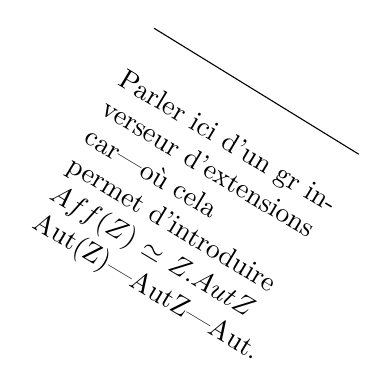
\begin{tikzpicture}
\draw (0,0.4)--(2.6,-1.2);
\node[anchor=north west,rotate=-31,align=left,text width=3.2cm,inner sep=0pt] at (-0.35,-0.1)
{\unsure{Parler} ici d'un gr inverseur d'extensions \unsure{car|où} cela permet d'introduire $\operatorname{Aff}(Z)\simeq Z.\operatorname{Aut}Z$ \deleted{\unsure{Aut(Z)|AutZ|Aut}}.};
\end{tikzpicture}}
\normalmarginpar

\[
\begin{aligned}
&\deleted{(\gamma,z)(\gamma',z')=(\gamma\gamma',\operatorname{int}(\gamma')^{-1}(z).z')}\\
&(z,\gamma)(\unsure{z'|{\mathcal Z}'},\gamma')=(z\operatorname{int}(\gamma)(z'),\gamma\gamma')
\end{aligned}
\]

% Lower-right note with its oblique divider and the short adjacent stroke.
\margin{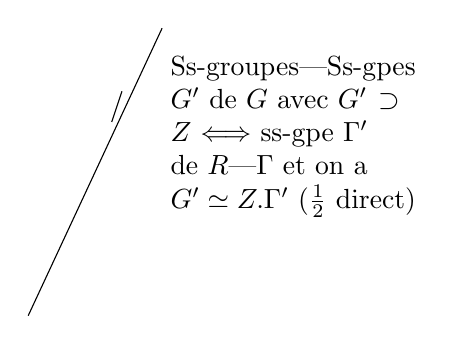
\begin{tikzpicture}
\draw (0,-3.5)--(1.7,0.15);
\draw (1.06,-1.04)--(1.19,-0.65);
\node[anchor=north west,align=left,text width=3.2cm,inner sep=0pt] at (1.8,-0.2)
{\unsure{Ss-groupes|Ss-gpes} $G'$ de $G$ avec $G'\supset Z$ $\Longleftrightarrow$ ss-gpe $\Gamma'$ de \deleted{\unsure{$R$|$\Gamma$}} et on a $G'\simeq\mathbb{Z}.\Gamma'$ ($\frac{1}{2}$ direct)};
\end{tikzpicture}}
% archive sheet number: 8
